
This chapter provides an overview of the project in \autoref{sec:overview}, outlines the necessary modifications to the existing project to execute ExpoSE on the execution platform in \autoref{sec:fwd-z3}, and presents the discovered system-imposed limitations in \autoref{sec:limits}. It then presents the initial idea in \autoref{sec:init-test-plain}. Some of them were contingent upon the platform on which the program was executed. In this case, an Apple MacBook Pro with an M1 Pro chip. 

\section{Overview}
\label{sec:overview}


ExpoSE functions as depicted in \autoref{fig:expose-struc} starting from a component referred to as the distributor to orchestrate the process of symbolic execution. The distributor facilitates the transmission of inputs to the executor, which, as its designation implies, executes the program under test utilizing these inputs. The execution of the program produces a trace, which is subsequently returned to the executor. From this trace, the path condition corresponding to the input is communicated to the SMT Solver. The SMT Solver solves the constraints and then transmits the resulting model back to the executor, enabling the executor to extrapolate alternative inputs. These alternative inputs are subsequently relayed to the distributor, thereby initiating the entire process again. In scenarios where multiple alternative inputs are generated, these inputs are executed concurrently.

For our case, the program under test is not just one script, but consists of both the server and the client, but also of the express model, the request model and the response model. 



\begin{figure}
  \centering
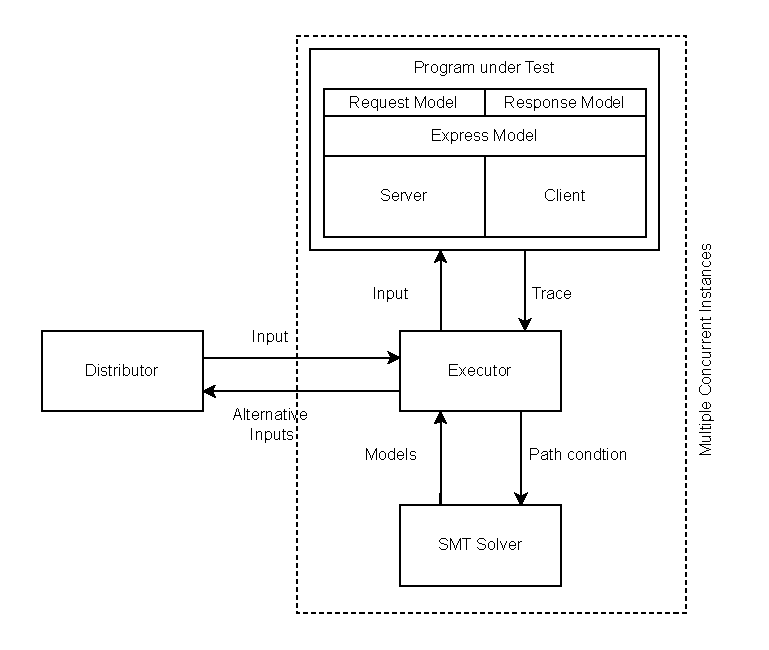
\includegraphics[width=0.7\textwidth]{exposeArchitectureDiagram.pdf}
 \caption[ExpoSE Architecture]{ExpoSE architecture structure, as depicted in \cite{loring_expose_2017}, modified to include the web application with the models for express, request, and response.}
     \label{fig:expose-struc}
\end{figure}


\FloatBarrier
\section{Forwarding Changes of Z3}
\label{sec:fwd-z3}
This section provides a short overview of the changes made to two of the four main parts that make up ExpoSE. Both were relatively simple in nature, but they were required to fix a Z3 specific internal error, that kept occurring and caused the execution to fail.

\subsection{Changes to Z3}
\label{sec:changes-z3}
As the forked repository of Z3 made for ExpoSE was almost 5 years old, and we noticed a null pointer exception in the C++ code, we decided to merge the changes from the original repository into the fork. There were almost 5000 commits since the last merge, and we hoped that the null pointer exception has been fixed meanwhile. 
The forwarding went smoothly, with two exceptions. Z3 now includes the type “Char Pointer”, which had to be added to the JavaScript portion of the binding creation.

The second exception was, that the Z3 API now provided a few more callbacks, which required parameters that were not implemented for JavaScript. 
We deleted these callbacks, as these would stop the generation of the bindings and of the dynamically linked library (DLL) of Z3.

\subsection{Changes to Z3JavaScript}
\label{sec:changes-z3js}
With the update to Z3 itself, we also had to update the Z3JavaScript project, as this defined the types for the JavaScript bindings. It turned out to be a simple issue of adding two new object types (a ParserContextObj and a SimplifierObj) of the type voidp, which is a pointer to the type void.


\section{System-imposed limitations}
\label{sec:limits}
In this section, we will explain the limitations imposed on the application, their consequences, and which of these consequences can or cannot be circumvented.
\subsection{JavaScript Version}
\label{sec:jsversion}
The hardest limitation of the application is that we have to stay in syntax constructs offered by the JavaScript version known as ES6 (or ECMA 2015).

This is a significant limitation, as it implies that we are unable to utilize an essential feature of contemporary JavaScript, specifically \textit{async} and \textit{await}. These two keywords refer to the asynchronous pattern that modern JavaScript employs. Without these, we will not be able to build a modern application, which is a major limitation for a server that might have to wait for resources to load or for a computation-intensive process. For these processes, we now have to rely on the practice of nesting callbacks. 




\subsection{Symbolic Addresses and Objects}
\label{sec:sym-obj}
While the other limits are specific to our use case, this issue is universal. Pointers can pose challenges for most symbolic execution engines, as highlighted in various studies, including those by \citet{cha_unleashing_2012}, \citet{coppa_rethinking_2017} and \citet{elkarablieh_precise_2009}.
Reasoning about the address of a variable poses an issue, as in theory, DSE would have to assume all possible addresses. 
\citet{elkarablieh_precise_2009} propose an approach that limits every pointer to a concrete memory region in which it remains symbolically, reducing the amount of possible memory addresses, which in theory is simple, but as itself proclaims “nontrivial to implement”. 
\citet{coppa_rethinking_2017} introduce the concept of \textbf{MemSight}, which allows the mapping of symbolic expressions to data, instead of instantiated addresses, reducing the need to concretize the symbolic memory addresses. 

\citet{cha_unleashing_2012} proposed a symbolic address, which concretizes writes and only the read is a symbolic operation. 
A similar approach was also taken for ExpoSE, as it concretizes the namespace a variable can occupy, and only its value is resolved symbolically.
ExpoSE initializes a symbolic object by reserving a namespace, concretizing it.


On execution, it then tracks every property access, updating the initial object with a new symbolic variable for the accessed property. 
If we consider this expression:\\
\lstinline[language=JavaScript]{const object = S$.symbol("object");}
This instruction initilizes the variable object as a new symbolic variable, without any indication that it is an object. 
Should ExpoSE now encounter a property access, i.e.
\lstinline[language=JavaScript]{if(object.field === "value")},
the property \lstinline[language=JavaScript]{object.field} gets initilized as a new symbolic variable
\lstinline[language=JavaScript]{object.field = S$.symbol("field");} 
and a path condition gets added, that \lstinline[language=JavaScript]{object} is, in fact, an object.\cite{loring_systematic_2021}

While this works in theory, it is incredibly costly, leading to an explosion of paths, due to the dynamically typed nature of JavaScript, thus adding one path condition per type just on encountering a property access. In black-box testing, where the program has no other option for reasoning about the kind of inputs the program takes, using completely symbolic objects does increase coverage and helps to find bugs.
In our case, however, where we have full access to the code and where we have knowledge of all input fields, this can be avoided by creating an object with possible properties already symbolically initialized. This can be done because all unused fields are simply ignored and not adding new path conditions. 
This means, instead of waiting for ExpoSE to find \lstinline{object.field}, we start with an object already containing the field, together with a seed indicating the type, as can be seen in 
\begin{lstlisting}[language=JavaScript]
const object = {
   "field": S$.symbol("field", "string"),
    "numberfield"; S$.symbol("numberfield", 10),
};
\end{lstlisting}




\subsection{External Packages}
\label{sec:externalpack}
Our last hard limit was the DSE engine assuming any imported package being part of the system under test. Although it was technically correct, this caused imported packages to be instrumented and execution branches being created, leading to a massive explosion in branches. While it could be used to find bugs and errors in these external packages as well, it did not offer any benefit for locating issues in the part of the web application we wanted to test. 
Hence, we opted out of using any external package for now.

\subsection{Dependency Issues}
\label{sec:dep-issues}
While this was not a limitation per se, it proved to be an issue with executing the tool chain of ExpoSE in the first place. When the codebase was created in 2017, almost all personal computers were x86-based. While ARM was already widespread in mobile devices, few personal computers were running on an ARM instruction set\footnote{We assume this to be the case, as even the \href{https://www.arm.com/-/media/global/company/investors/Arm\%20Strategic\%20Review\%20-\%202017.pdf?revision=8473a535-6f7e-4ce5-85fe-0eb6f1f75487&la=en}{investor report} in 2017 does not mention them}. Therefore, little to no effort was spent on supporting it. 
With the release of the M1 processor by Apple, this was no longer the case.
This meant that the ARM instruction set went from being rarely supported to wide-spread use.
When we started working on this thesis, we noticed the lack of support. The project required Node version 14, and the package ffi-napi\footnote{https://www.npmjs.com/package/ffi-napi}, that provided the ability to create C bindings, which were used in Z3, required Node 16 or higher.
Upgrading the node version would in turn create an error in ffi-napi for the ARM-based M processors\footnote{As reported in issue https://github.com/node-ffi-napi/node-ffi-napi/issues/248}.\\
While working on this project, the issue got resolved by an update to ffi-napi.

\section{HTTP in Symbolic Execution}
\label{sec:http}
When working with web applications, there are multiple components that have to be taken care of. The internal processing, the storing and retrieving of data, and most importantly, the communication between server and client.
This communication required leads to a dilemma in symbolic execution, as for it to function properly, it needs to hold the symbolic state across the many processing layers between client and server. 

The requests and responses are handled at the operating system level, converted into binaries, leaving the context to a symbolic execution engine can handle. Most already face the issue of being based on a singular programming language. If, for example, we create a JavaScript request, we can have a symbolic state only as it exists in this context. Once it leaves the context of a JavaScript application, we would require an engine that supports multiple languages and can also operate on a system level. On the receiving end, the engine has to reverse this process, and continue with the incoming symbolic request.


There have been efforts to support this cross-language and cross-platform dynamic symbolic execution. \citet{bucur_prototyping_2014-1} introduced \textbf{Chef}, which is a tool to use the interpreter as an engine specification, creating a symbolic interpreter, in contrast to an engine that gets executed instead. Built on top of \textbf{S\textsuperscript{2}E}\cite{chipounov_s2e_2011}, which symbolically executes a virtual machine with all of its parts such as the OS kernel, and programs, CHEF has the potential to track the state of an input across multiple systems.


However, as these approaches are highly resource intensive, using a cross-platform approach seemed impractical for the purpose of our goal. This led us to the solution we will be using for our tests; we bypass the communication between client and server completely, by injecting the server into the client, or vice versa, depending on the server structure (more on that in \autoref{chapter:express}). With that, we would have the full symbolic state of the execution, the data would not need to be transformed, and could simply be handed over to the request and response processing on server- and client-side. 
We deemed this the correct approach because it achieves the goal of a symbolic communication we would get with a cross-platform approach, but less costly.


\section{Initial Testing of a Plain JavaScript Application}
\label{sec:init-test-plain}
After addressing all the fundamental issues, we began by creating a small server in plain JavaScript to explore whether it is possible to generate requests, process them, and return the correct response for the request. For example, a \texttt{GET} request with the URL \lstinline[language=JavaScript]+"/test"+ is handled by a \texttt{GET} route registered as \lstinline[language=JavaScript]{"/test"}, and not incorrectly by the \texttt{POST} route. 

\subsection{Idea}
\label{sec:idea}

The objective was to construct a plain JavaScript server by utilizing the http package's method “createServer” and subsequently eliminating all components that depend on http, thus skipping the actual server-client connection.
We had two goals for this: 
\begin{enumerate}
    \item  We created a server that had both static and variable routes, notably one route that consisted only of a regular expression, to test whether all routes could be found by the symbolic variable for the path alone.
    \item  We also implemented a short test for injecting code into the response, by asserting that the client cannot send any script tag \lstinline[language=JavaScript]{<script><\script>} in the request data, while asserting that it has to be a valid email. Which in turn meant ExpoSE has to try to violate the assertion by creating inputs that contain a script tag and are no valid emails. 
\end{enumerate}
For the client side we created a bare-bones client that was generating the symbolic request, and passed it over to the server by calling the onRequest method of the server, which gets called whenever a request is sent, bypassing HTTP. 

\subsection{Evaluation}
This small test application was able to prove that it is indeed possible to test a server with ExpoSE by fulfilling both requirements stated in \autoref{sec:idea}. Finding all the request routes within the server was straightforward, with one minor drawback: the regular expression route was not functional in a switch-case construct due to its use as a literal and not as a regular expression to match a string. 
The second objective was only moderately successful, as, despite demonstrating theoretically that the generation of a string containing a script tag works, it often exceeded the timeout limit, with a few exceptions in a test of 50 runs, where a matching string was immediately generated.

Despite this, we deemed the initial test application a success, as it strongly suggested that it is possible to test a server, explore all possibly routes and locate issues in the validation, data processing and usage of this data. Hence, we moved on from plain JavaScript to the usage of a framework, in our case, Express.
